%%%%%%%%%%%%%%%%%%% vorlage.tex %%%%%%%%%%%%%%%%%%%%%%%%%%%%%
%
% Beispiel-Vorlage zur Erstellung von Projekt-Dokumentationen
%
% Benutzen Sie bitte diese Datei um Ihre Dokumente zu erstellen
%
%%%%%% erstellt anhand svmono-Springer-Verlag-Vorlage %%%%%%%%%
%Hier hat Emolotow etwas Senf hinterlassen =D

%%%%%%%%%%%%%%%%%%%%%%%%%%%%%%%%%%%%%%%%%%%%%%%%%%%
\documentclass[envcountsame,envcountchap, deutsch]{i-studis}


\usepackage{makeidx}         % Erlaubt die Erzeugung eines Index-Verzeichnisses
\usepackage{multicol}        % Zweispaltiger Index-Verzeichnis
%\usepackage[bottom]{footmisc} % Erzeugung von Fu�noten nur beim Bedarf einbinden
\usepackage{caption}
\usepackage{subcaption}
%\usepackage{wrapfig}

%%-----------------------------------------------------
%\newif\ifpdf
%\ifx\pdfoutput\undefined
%\pdffalse
%\else
%\pdfoutput=1
%\pdftrue
%\fi
%%--------------------------------------------------------
%\ifpdf
\usepackage[pdftex]{graphicx}
\usepackage[pdftex,plainpages=false]{hyperref}
%\else
%\usepackage{graphicx}
%\usepackage[plainpages=false]{hyperref}
%\fi
%%-----------------------------------------------------
\usepackage{color}	% Farbverwaltung
%\usepackage{ngerman} % Neue deutsche Rechtsschreibung
\usepackage[english, ngerman]{babel}
\usepackage[latin1]{inputenc} % Erm�glicht Umlaute-Darstellung
%\usepackage[utf8]{inputenc}  % Ermöglicht Umlaute-Darstellung unter Linux (je nach verwendetem Format)
%-----------------------------------------------------
\usepackage{listings} % Code-Darstellung
\usepackage{media9} %Gif and Movie support
\lstset
{% general command to set parameter(s)
	basicstyle=\scriptsize, % print whole listing small
	keywordstyle=\color{blue}\bfseries,
	% underlined bold black keywords
	identifierstyle=, % nothing happens
	commentstyle=\color{red}, % white comments
	stringstyle=\ttfamily, % typewriter type for strings
	showstringspaces=false, % no special string spaces
	framexleftmargin=7mm, 
	tabsize=3,
	showtabs=false,
	frame=single, 
	rulesepcolor=\color{blue},
	numbers=left,
	linewidth=146mm,
	xleftmargin=8mm
}
\usepackage{textcomp} % celsius - Darstellung
\usepackage{
amssymb,
amsfonts,
amstext,
amsmath
} % Mathematische Symbole
\usepackage[german, ruled, vlined]{algorithm2e}
\usepackage[a4paper]{geometry} %Andere Formatierung
\usepackage{bibgerm}
\usepackage{array}
\hyphenation{Ele-men-tar-ob-jek-te  ab-ge-tas-tet Aus-wer-tung House-holder-Matrix Le-ast-Squa-res-Al-go-ri-th-men} %Silbentrennung bei falschen Trennung angeben
\setlength{\textheight}{1.1\textheight}
\pagestyle{myheadings} % Erzeugt selbstdefinierte Kopfzeile
\makeindex % Index-Erstellung

% Ab hier beginnt das eigentliche Dokument.
%--------------------------------------------------------------------------
\begin{document}

%------------------------- Titelblatt -------------------------------------
\title{\textbf{Wo geht's lang...?}}
\subtitle{Analyse von Wegfindealgorithmen und ihr Einsatz 
im Gamedesign}
%---- Die Art der Dokumentation kann hier ausgew�hlt werden---------------
%\project{Master Abschlussarbeit}
%\project{Master Projektstudium}
%\project{Bachelor Abschlussarbeit}
%\project{Projektarbeit}
%\project{Seminar zur Vorlesung ...}
\project{Wissenschaftliches Arbeiten}
%--------------------------------------------------------------------------
\supervisor{\\Prof. Dr. J. Lohscheller, \\
    Prof. Dr. A. Lux,  \\
     Prof. Dr. K. M�rthesheimer, \\
      Prof. Dr. N. Rudolph} % Betreuer der Arbeit
\author{Boos, Jeremias \\ Neugebauer, Manuel} %Autor der Arbeit
\address{Trier, } % Im Zusammenhang mit dem Datum wird hinter dem Ort ein Komma angegeben
\submitdate{22.05.2014} % Abgabedatum
%\begingroup
%  \renewcommand{\thepage}{title}
%  \mytitlepage
%  \newpage
%\endgroup
\begingroup
  \renewcommand{\thepage}{Titel}
  \mytitlepage
  \newpage
\endgroup
%--------------------------------------------------------------------------
\frontmatter 
%--------------------------------------------------------------------------
\danksagung

Dank an ... %Danksagungen
%\preface

Ein Vorwort ist nicht unbedingt n�tig. Falls Sie ein Vorwort schreiben, so ist dies der Platz, um z.B. die
Firma vorzustellen, in der diese Arbeit entstanden ist, oder einigen Leuten zu danken, die in irgendeiner
Form positiv zur Entstehung dieser Arbeit beigetragen haben. Auf keinen Fall sollten Sie im Vorwort die
Aufgabenstellung n�her erl�utern oder vertieft auf technische Sachverhalte eingehen.
%%%%%%%%%%%%%%%%%%%%%% Kurzfassung.tex %%%%%%%%%%%%%%%%%%%%%%%%%%%%%%%%%%%%%
%
% sample preface
%
% Use this file as a template for your own input.
%
%%%%%%%%%%%%%%%%%%%%%%%% Spinner-Verlag %%%%%%%%%%%%%%%%%%%%%%%%%%

\kurzfassung

%% Schreiben Sie Ihre Kurzfassung hierher
A* ist der meistbenutzte Algorithmus in Sachen Wegfindung. Es werden die Funktionen und Berechnungen dahinter erkl�rt. Auch wird auf die Grundlage und Weiterentwicklung dessen eingegangen. 
\\[3ex]

%% Please write your preface here
%this is just to troll the reviewer
\noindent
A* is the most commonly used algorythm for pathfinding. Here we are, to praise the holy god of A*, that he will crush our enemys and bless our code. Hail to the glorious algorythm who gives us CPU time. \\obey!!

 % Kurzfassung Deutsch/English
\tableofcontents %Inhaltsverzeichnis - notwendig
\listoffigures % Abbildungsverzeichnis - optional
%\listoftables % Tabellenverzeichnis- optional
%--------------------------------------------------------------------------
\mainmatter                        %Hauptteil (ab hier arab. Seitenzahlen)
%--------------------------------------------------------------------------
% Kapitell werden einzeln abgespeichert und hier eingef�gt
\chapter{Einleitung}
%Begonnen werden soll mit einer Einleitung zum Thema: z.B. Hintergrund und Ziel
%(was, warum).
In vielen Computerspielen ist eine Funktion von N�ten um Einheiten und Charaktere ans Ziel zu f�hren. Egal in welchen Genre, wenn sich der Computer in einer simulierten Umgebung effizient zurecht finden soll, wird ein Wegfindealgorithmus ben�tigt. Um Umwege und unnat�rlich wirkendes Verhalten zu vermeiden, bietet sich ein heuristischer, Graphen basierter Algorithmus an.
Dieser hat sich als effizienteste L�sung f�r Wegfindeprobleme erwiesen.\\
Nicht nur in Civilization, wo die Funktionsweise dem Spieler als ein Zentrales Spielelement bewusst wird, finden solche Algorithmen Verwendung. Auch Genres scheinbar abseits taktischer Tiefe, wie Beispielsweise MMORPGS oder Shootern w�ren ohne dieselben nicht realisierbar.\\

%In vielen Jahren der Spieleentwicklung hat sich A*(A-Stern) als der Effizienteste seiner Art herauskristallisiert.
Wegen seiner einfachen Implementierung und seines hohen Effizienzgrades hat sich A*(A-Stern) als Geeignetster seiner Art bew�hrt. Daher wird heute kaum noch auf andere L�sungen zur�ckgegriffen um entsprechende Probleme zu bew�ltigen. In so fern wird sich diese Arbeit mit den Eigenschaften und der Umsetzung in Programmen von A* befassen.


\chapter {Dijkstra}
Der auf der Graphentheorie beruhende Dijkstra bildet die Grundlage zu A*. Er wurde vom gleichnamigen Professor im Jahr 1959 in einem Lehrbuch erl�utert.\footnote{\cite{EWD:NumerMath59}} Es ist der �blichste Algorithmus, der f�r Netzwerkrouting eingesetzt wird.\footnote{\cite{tanenbaum:CN}} \\

\section {Funktionsweise}
Die Knoten im Dijkstra-Algorithmus haben folgende Eigenschaften:
\begin{itemize}
	\item Die Kosten des ersten Knotens betragen 0.
	\item Sonstige Knotenkosten akkumulieren sich aus den Kosten der Vorg�ngerknoten.
	\item Die Unbekannten ausgenommen, hat jeder Knoten ein Vorg�nger, der die bisher k�rzeste Verbindung zum ersten Knoten darstellt.
	\item fertig untersuchte Knoten werden ignoriert
\end{itemize}

\newpage
\subsection{Iterative Vorgehensweise}

\begin{enumerate}
	\item Die Knoten werden in 3 Listen sortiert
	\begin{itemize}
		\item unbekannte Knoten
		\item zu untersuchende Knoten
		\item fertig untersuchte Knoten
	\end{itemize}
	\item Am Anfang ist der Startknoten als "'zu untersuchend"' markiert, alle Anderen sind unbekannt. \ref{Schritt 0}
	\item Aus der Liste der zu untersuchenden Knoten wird nun jener erw�hlt, welcher am wenigsten Kosten verursacht. \item Dieser wird nun in die Liste der fertig untersuchten Knoten verschoben. \ref{Schritt 7}
	\begin{itemize}
		\item War dies der Zielknoten, so ergibt sich als Ergebnis der Weg vom Anfang bis zum Ziel. \ref{Schritt 25}
		\item Wenn nicht, so werden die unbekannten, direkt verbundenen Knoten in die Liste der zu Untersuchenden angef�gt. Dabei werden die Kosten der Knoten ermittelt und der Vorg�ngerknoten gesetzt.(\ref{Schritt 1} - \ref{Schritt 6})\\ 
		Es gilt:\\
		$Knotenkosten=Weg+Kante$\\
		$D(k_{i})=D(k_{i-1})+Kantenkosten$
		\\
		Falls f�r den Knoten schon einmal Kosten ermittelt wurden, so wird der niedrigste Betrag �bernommen.
	\end{itemize}
\end{enumerate}
Schritte 3 und 4 werden wiederholt, bis die Liste der zu untersuchenden Knoten leer ist. Bei einem erfolgreichen Ablauf kann vom Ziel bis zum Startknoten der k�rzeste Weg verfolgt werden.(\ref{Schritt 1} - \ref{Schritt 25})\\
Falls das Ziel nicht erreicht wurde, gibt es keinen Weg �ber die angegebenen Knoten.\\
\newpage
\subsection{Ein kleines Beispiel}

\newcounter{Schritt}
\setcounter{Schritt}{0}

\begin{figure}
\centering
\caption{Schritte vom Start bis zum Ende der Untersuchung der Nachbarknoten von 2}
\label{Schritt 0 - 11}
\begin{subfigure}[b]{0.24\textwidth} %[hbtp]
	\centering
		\includegraphics[width=\textwidth]{images/Dijkstra-Beispiel/\arabic{Schritt}.png}
	\caption{Schritt \arabic{Schritt}}
	\label{Schritt \arabic{Schritt}}
	\addtocounter{Schritt}{1}
\end{subfigure}
\hfill
\begin{subfigure}[b]{0.24\textwidth} %[hbtp]
		\includegraphics[width=\textwidth]{images/Dijkstra-Beispiel/\arabic{Schritt}.png}
	\caption{Schritt \arabic{Schritt}}
	\label{Schritt \arabic{Schritt}}
	\addtocounter{Schritt}{1}
\end{subfigure}
\hfill
\begin{subfigure}[b]{0.24\textwidth} %[hbtp]
\centering
		\includegraphics[width=\textwidth]{images/Dijkstra-Beispiel/\arabic{Schritt}.png}
	\caption{Schritt \arabic{Schritt}}
	\label{Schritt \arabic{Schritt}}
	\addtocounter{Schritt}{1}
\end{subfigure}
\hfill
\begin{subfigure}[b]{0.24\textwidth} %[hbtp]
\centering
		\includegraphics[width=\textwidth]{images/Dijkstra-Beispiel/\arabic{Schritt}.png}
	\caption{Schritt \arabic{Schritt}}
	\label{Schritt \arabic{Schritt}}
	\addtocounter{Schritt}{1}
\end{subfigure}
\\
\begin{subfigure}[b]{0.24\textwidth} %[hbtp]
	\centering
		\includegraphics[width=\textwidth]{images/Dijkstra-Beispiel/\arabic{Schritt}.png}
	\caption{Schritt \arabic{Schritt}}
	\label{Schritt \arabic{Schritt}}
	\addtocounter{Schritt}{1}
\end{subfigure}
\hfill
\begin{subfigure}[b]{0.24\textwidth} %[hbtp]
		\includegraphics[width=\textwidth]{images/Dijkstra-Beispiel/\arabic{Schritt}.png}
	\caption{Schritt \arabic{Schritt}}
	\label{Schritt \arabic{Schritt}}
	\addtocounter{Schritt}{1}
\end{subfigure}
\hfill
\begin{subfigure}[b]{0.24\textwidth} %[hbtp]
\centering
		\includegraphics[width=\textwidth]{images/Dijkstra-Beispiel/\arabic{Schritt}.png}
	\caption{Schritt \arabic{Schritt}}
	\label{Schritt \arabic{Schritt}}
	\addtocounter{Schritt}{1}
\end{subfigure}
\hfill
\begin{subfigure}[b]{0.24\textwidth} %[hbtp]
\centering
		\includegraphics[width=\textwidth]{images/Dijkstra-Beispiel/\arabic{Schritt}.png}
	\caption{Schritt \arabic{Schritt}}
	\label{Schritt \arabic{Schritt}}
	\addtocounter{Schritt}{1}
\end{subfigure}
\\
\begin{subfigure}[b]{0.24\textwidth} %[hbtp]
	\centering
		\includegraphics[width=\textwidth]{images/Dijkstra-Beispiel/\arabic{Schritt}.png}
	\caption{Schritt \arabic{Schritt}}
	\label{Schritt \arabic{Schritt}}
	\addtocounter{Schritt}{1}
\end{subfigure}
\hfill
\begin{subfigure}[b]{0.24\textwidth} %[hbtp]
		\includegraphics[width=\textwidth]{images/Dijkstra-Beispiel/\arabic{Schritt}.png}
	\caption{Schritt \arabic{Schritt}}
	\label{Schritt \arabic{Schritt}}
	\addtocounter{Schritt}{1}
\end{subfigure}
\hfill
\begin{subfigure}[b]{0.24\textwidth} %[hbtp]
\centering
		\includegraphics[width=\textwidth]{images/Dijkstra-Beispiel/\arabic{Schritt}.png}
	\caption{Schritt \arabic{Schritt}}
	\label{Schritt \arabic{Schritt}}
	\addtocounter{Schritt}{1}
\end{subfigure}
\hfill
\begin{subfigure}[b]{0.24\textwidth} %[hbtp]
\centering
		\includegraphics[width=\textwidth]{images/Dijkstra-Beispiel/\arabic{Schritt}.png}
	\caption{Schritt \arabic{Schritt}}
	\label{Schritt \arabic{Schritt}}
	\addtocounter{Schritt}{1}
\end{subfigure}
\end{figure}
\begin{figure}
\caption{2 wird in die "'abgeschlossen Liste"' integriert, bis "'Pfad gefunden"'}
\label{Schritt 12 - 26}
\begin{subfigure}[b]{0.24\textwidth} %[hbtp]
	\centering
		\includegraphics[width=\textwidth]{images/Dijkstra-Beispiel/\arabic{Schritt}.png}
	\caption{Schritt \arabic{Schritt}}
	\label{Schritt \arabic{Schritt}}
	\addtocounter{Schritt}{1}
\end{subfigure}
\hfill
\begin{subfigure}[b]{0.24\textwidth} %[hbtp]
		\includegraphics[width=\textwidth]{images/Dijkstra-Beispiel/\arabic{Schritt}.png}
	\caption{Schritt \arabic{Schritt}}
	\label{Schritt \arabic{Schritt}}
	\addtocounter{Schritt}{1}
\end{subfigure}
\hfill
\begin{subfigure}[b]{0.24\textwidth} %[hbtp]
\centering
		\includegraphics[width=\textwidth]{images/Dijkstra-Beispiel/\arabic{Schritt}.png}
	\caption{Schritt \arabic{Schritt}}
	\label{Schritt \arabic{Schritt}}
	\addtocounter{Schritt}{1}
\end{subfigure}
\hfill
\begin{subfigure}[b]{0.24\textwidth} %[hbtp]
\centering
		\includegraphics[width=\textwidth]{images/Dijkstra-Beispiel/\arabic{Schritt}.png}
	\caption{Schritt \arabic{Schritt}}
	\label{Schritt \arabic{Schritt}}
	\addtocounter{Schritt}{1}
\end{subfigure}
\\
\begin{subfigure}[b]{0.24\textwidth} %[hbtp]
	\centering
		\includegraphics[width=\textwidth]{images/Dijkstra-Beispiel/\arabic{Schritt}.png}
	\caption{Schritt \arabic{Schritt}}
	\label{Schritt \arabic{Schritt}}
	\addtocounter{Schritt}{1}
\end{subfigure}
\hfill
\begin{subfigure}[b]{0.24\textwidth} %[hbtp]
		\includegraphics[width=\textwidth]{images/Dijkstra-Beispiel/\arabic{Schritt}.png}
	\caption{Schritt \arabic{Schritt}}
	\label{Schritt \arabic{Schritt}}
	\addtocounter{Schritt}{1}
\end{subfigure}
\hfill
\begin{subfigure}[b]{0.24\textwidth} %[hbtp]
\centering
		\includegraphics[width=\textwidth]{images/Dijkstra-Beispiel/\arabic{Schritt}.png}
	\caption{Schritt \arabic{Schritt}}
	\label{Schritt \arabic{Schritt}}
	\addtocounter{Schritt}{1}
\end{subfigure}
\hfill
\begin{subfigure}[b]{0.24\textwidth} %[hbtp]
\centering
		\includegraphics[width=\textwidth]{images/Dijkstra-Beispiel/\arabic{Schritt}.png}
	\caption{Schritt \arabic{Schritt}}
	\label{Schritt \arabic{Schritt}}
	\addtocounter{Schritt}{1}
\end{subfigure}
\\
\begin{subfigure}[b]{0.24\textwidth} %[hbtp]
	\centering
		\includegraphics[width=\textwidth]{images/Dijkstra-Beispiel/\arabic{Schritt}.png}
	\caption{Schritt \arabic{Schritt}}
	\label{Schritt \arabic{Schritt}}
	\addtocounter{Schritt}{1}
\end{subfigure}
\hfill
\begin{subfigure}[b]{0.24\textwidth} %[hbtp]
		\includegraphics[width=\textwidth]{images/Dijkstra-Beispiel/\arabic{Schritt}.png}
	\caption{Schritt \arabic{Schritt}}
	\label{Schritt \arabic{Schritt}}
	\addtocounter{Schritt}{1}
\end{subfigure}
\hfill
\begin{subfigure}[b]{0.24\textwidth} %[hbtp]
\centering
		\includegraphics[width=\textwidth]{images/Dijkstra-Beispiel/\arabic{Schritt}.png}
	\caption{Schritt \arabic{Schritt}}
	\label{Schritt \arabic{Schritt}}
	\addtocounter{Schritt}{1}
\end{subfigure}
\hfill
\begin{subfigure}[b]{0.24\textwidth} %[hbtp]
\centering
		\includegraphics[width=\textwidth]{images/Dijkstra-Beispiel/\arabic{Schritt}.png}
	\caption{Schritt \arabic{Schritt}}
	\label{Schritt \arabic{Schritt}}
	\addtocounter{Schritt}{1}
\end{subfigure}
\\
\begin{subfigure}[b]{0.24\textwidth} %[hbtp]
	\centering
		\includegraphics[width=\textwidth]{images/Dijkstra-Beispiel/\arabic{Schritt}.png}
	\caption{Schritt \arabic{Schritt}}
	\label{Schritt \arabic{Schritt}}
	\addtocounter{Schritt}{1}
\end{subfigure}
\hfill
\begin{subfigure}[b]{0.24\textwidth} %[hbtp]
		\includegraphics[width=\textwidth]{images/Dijkstra-Beispiel/\arabic{Schritt}.png}
	\caption{Schritt \arabic{Schritt}}
	\label{Schritt \arabic{Schritt}}
	\addtocounter{Schritt}{1}
\end{subfigure}
\hfill
\begin{subfigure}[b]{0.24\textwidth} %[hbtp]
\centering
		\includegraphics[width=\textwidth]{images/Dijkstra-Beispiel/\arabic{Schritt}.png}
	\caption{Schritt \arabic{Schritt}}
	\label{Schritt \arabic{Schritt}}
	\addtocounter{Schritt}{1}
\end{subfigure}
\hfill
\end{figure}
{\small{\it{Quelle: http://upload.wikimedia.org/wikipedia/commons/5/57/Dijkstra\_Animation.gif}}}
\chapter{A*}
Der Algorithmus von Dijkstra stellte sich als zufriedenstellend f�r den Netzwerkverkehr heraus. Aber f�r die Anforderungen, die KI-Entwickler Ende der sechziger Jahre, durch das Aufkommen von Computerspielen, zu bew�ltigen hatten war er einfach nicht geeignet. Dijkstra ist klar im Vorteil, wenn eine Strecke �ber bekannte Punkte mit konstanten L�ngen zur�ck gelegt werden soll. Aber sobald es m�glich ist die Kosten vom aktuelle Knoten zum Ziel zu sch�tzen, kann die Wegfindung optimiert werden.\\
A* ist demnach kein komplett neues Verfahren, sondern nur eine Optimierung des urspr�nglichen Algorithmus hinsichtlich dieser Punkte. Das wird besonders deutlich, wenn A* gegen eine Wand l�uft. Hier gleicht sich der Sch�tzwert, f�r neue Knoten, welche vermeidlich nahe am Ziel sind mit den ehemals h�heren Kosten der Knoten am Startpunkt an. So wird, je nach Implementierung, ein Feld nach dem anderen besucht, bis der Pfad nicht mehr blockiert ist.
Eine Besonderheit von A* ist, dass er optimal effizient eine L�sung findet - diese ist gleichzeitig der g�nstigste Weg.
\\ Er ist, unter den selben Ausgangsbedingungen (Heuristik), in seiner Geschwindigkeit, kombiniert mit jener Genauigkeit nicht mehr zu �bertrumpfen.\footnote{ \url{http://de.wikipedia.org/w/index.php?title=A*-Algorithmus\&oldid=129862855}}\\
Dazu kommt, dass die Heuristik dahingehend modifizierbar ist, A* schneller zum Ziel finden zu lassen. Dieser Weg wird voraussichtlich nicht der optimale sein. So wird Rechenzeit auf Kosten der Genauigkeit gewonnen.

\section{Funktionsweise}
Vor jedem Schritt werden die anliegenden Knoten �berpr�ft. Der Computer berechnet zuerst, wie bei Dijkstra, die bisher zur�ckgelegten Kosten. Zus�tzlich kommt nun hinzu, dass die Punkte noch einen Sch�tzwert erhalten, wie weit sie vom Ziel entfernt sind.\\
Zur Formel kommt dies nun als der Faktor $h(k)$.\\
Es gilt nun:\\
$F(k)=D(k)+h(k)$

\section{Beispiel}

\setcounter{Schritt}{1}

\begin{figure}
\centering
\caption{Vorgehensweise von A*}

\label{Schritt 1 - 5}

\begin{tabular}{c c}
\begin{subfigure}[b]{0.45\textwidth} %[hbtp]
	\centering
		\includegraphics[width=\textwidth]{images/A-Stern-Beispiel/aStar(\arabic{Schritt}).jpg}
	\caption{Ausgangssituation Start(Gr�n) und Ziel(Rot) werden durch das Hindernis(Blau) getrennt.}
	\label{A-Stern-Schritt \arabic{Schritt}}
	\addtocounter{Schritt}{1}
\end{subfigure}
&
\begin{subfigure}[b]{0.45\textwidth} %[hbtp]
	\centering
		\includegraphics[width=\textwidth]{images/A-Stern-Beispiel/aStar(\arabic{Schritt}).jpg}
	\caption{Untersuchen der Nachbarknoten vom Startpunkt aus. Oben links die gesch�tzten Gesamtkosten. Unten links die bisherigen Wegkosten. Unten rechts die gesch�tzte Entfernung.}
	\label{A-Stern-Schritt \arabic{Schritt}}
	\addtocounter{Schritt}{1}
\end{subfigure}
\\
\begin{subfigure}[b]{0.45\textwidth} %[hbtp]
	\centering
		\includegraphics[width=\textwidth]{images/A-Stern-Beispiel/aStar(\arabic{Schritt}).jpg}
	\caption{Die blaue Umrahmung zeigt die besuchten Knoten an. Hier endete die Suche in einer Wand. Nun wird der g�nstigste Knoten aus der Liste genommen.}
	\label{A-Stern-Schritt \arabic{Schritt}}
	\addtocounter{Schritt}{1}
\end{subfigure}
&
\begin{subfigure}[b]{0.45\textwidth} %[hbtp] 
	\centering
		\includegraphics[width=\textwidth]{images/A-Stern-Beispiel/aStar(\arabic{Schritt}).jpg}
	\caption{Der Zielknoten wurde gefunden und wird in die Liste der abgeschlossenen Knoten mit eingereiht.}
	\label{A-Stern-Schritt \arabic{Schritt}}
	\addtocounter{Schritt}{1}
\end{subfigure}
\\
\multicolumn{2}{ c  }{
\begin{subfigure}[b]{0.45\textwidth} %[hbtp]
	\centering
		\includegraphics[width=\textwidth]{images/A-Stern-Beispiel/aStar(\arabic{Schritt}).jpg}
	\caption{Nun kann der Weg vom Ziel aus durch die Verweise der einzelnen Knoten auf die Vorg�ngerknoten gebildet werden.}
	\label{A-Stern-Schritt \arabic{Schritt}}
	\addtocounter{Schritt}{1}
\end{subfigure}}
\end{tabular}
\\{\small{\it{Quelle:\cite{Les:06}}}}
\end{figure}


 

\chapter{Vergleich der beiden Algorithmen}

Beim Betrachten der beiden Algorithmen f�llt auf,
dass Worst- und Best-Case Situationen absolut identische Effizienzgrade haben.\\
Der Best-Case ist nat�rlich der Fall, in dem direkt in der ersten Iteration das Ziel gefunden wurde.\\
Der Worst-Case dem entsprechend, wenn das Ziel nicht zu finden, oder der letzte erreichbare Knoten ist.\\
Das zeigt, dass die Verbesserungen, welche A* von Dijkstras Algorithmus unterscheiden, nur ins Auge springen, wenn die Wegkosten gesch�tzt werden k�nnen.
Ein offenes Feld mit diversen einfachen Hindernissen ist demnach mehr geeignet als ein Labyrinth, welches nur wenige Strecken zum Ausgang zu l�sst.\\
\newpage
Wie auf \ref{DvsA} zu sehen, kann eine gleiche Ausgangssituation unterschiedlich schnell gel�st werden. Da Dijkstra keine Pr�ferenzen beim W�hlen der Knoten hat, sucht er alle Kanten, unabh�ngig von der Entfernung ab. \\
A* Stern hingegen besucht deutlich weniger Knoten. In dieser Situation lief er zuerst in das Hindernis. Verhielt sich anschlie�end wie Dijkstra, bis ein Weg um das Hindernis gefunden wurde. Wie in \ref{lastFrameA} und \ref{lastFrameD} zu sehen.


\begin{figure}
\centering
\caption{Dikstra Vergleich A*}
\label{DvsA}
%\caption{Dikstra Vergleich A*}
\begin{subfigure}[b]{0.5\textwidth} %[hbtp]
	\centering
		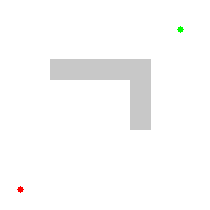
\includegraphics[width=\textwidth]{images/progress_Path_animation_firstframe.png}
	\caption{Ausganssituation}
	\label{Frame1}

\end{subfigure}
\\
\begin{subfigure}[b]{0.49\textwidth} %[hbtp]
	\centering
		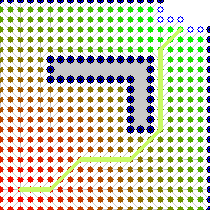
\includegraphics[width=\textwidth]{images/progress_Dijkstras_animation_lastframe.png}
	\caption{Endsituation Dijkstra}
		\label{lastFrameD}
\end{subfigure}
\begin{subfigure}[b]{0.49\textwidth} %[hbtp]
	\centering
		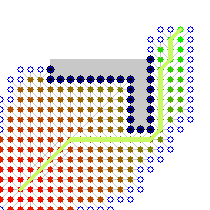
\includegraphics[width=\textwidth]{images/progress_Astar_animation_lastframe.png}
	\caption{Endsituation A*}
		\label{lastFrameA}
\end{subfigure}
{\small{\it{Quelle: http://upload.wikimedia.org/wikipedia/commons/5/5d/Astar\_progress\_animation.gif}}}\\
{\small{\it{Quelle: http://upload.wikimedia.org/wikipedia/commons/2/23/Dijkstras\_progress\_animation.gif}}}
\end{figure}

\chapter{Implementierung in Computerspielen}
In der Praxis werden in heutigen Spielen Mobs nicht mehr einfach �ber eine 2-Dimensionale Oberfl�che, mit n Knoten, ans Ziel gelotst. In 3D Spielen ist nicht nur die Frage wie optimal, sondern auch wie nat�rlich sich die Figur zum Zielpunkt bewegt.
%In der dritten Dimension m�ssen, sich scheinbar �berlappende Wege, (z.B. unterschiedliche Stockwerke) auf eine zweidimensionale Ebene herunter gebrochen werden.\\
\section{Drahtgitter}
Ein Drahtgitter (oder auch Grid) ist wie das Blatt eines Rechenblockes, welches �ber eine Karte gelegt wird. Diese Technik findet heute noch bei Strategietiteln Verwendung und war in den Neunzigern quasi Standard f�r alle Spiele aus der Vogelperspektive.
Den Feldern k�nnen Eigenschaften zugewiesen werden. So kann man bestimmen, ob sich die Figur vor, hinter oder gar nicht �ber ein Objekt bewegen kann.\\
Je nach Bedarf k�nnen so auch Felder mit h�heren oder niedrigeren Bewegungskosten, Schaden oder Heilung und anderen Boni und Mali versehen werden.
\newpage
\section{Navigation Meshes}
Hier handelt es sich um Polygone, welche bei Erstellung der Karte auf den Boden gelegt werden, um die begehbare Zone auszuweisen. Gewisserma�en werden aus den Verbindungslinien der Knoten -bei Dijkstra- breite Stra�en. So wird der ehemalige Seilt�nzer, der sich auf einer festen Linie von A nach B bewegt ein Fahrradfahrer mit Spielraum auf der Strecke.\\
Zus�tzlich kommt hinzu, dass jedes Dreieck der Polygone als Knoten verwertet werden kann. Dies wird generell nur ausgenutzt, wenn sich neue Routen erschlie�en und neue Wegfinde-Entscheidungen zu treffen sind. Daraus erschlie�t sich auch die Dynamik dieser Felder.\\
Es muss beachtet werden, diese Meshes um eine weitere Dimension zu erweitern, soll sich der Mob komplett in den Raum bewegen. Also f�r den Fall, er taucht oder fliegt.

\begin{figure}
	\centering
		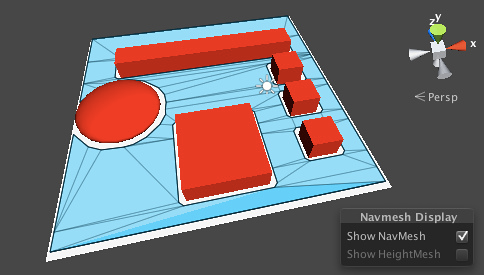
\includegraphics[width=0.3\textwidth]{images/Navmeshes-2.png}
	
	\label{navmesh}
	\caption{Navmesh Beispiel aus Unity3D}
	{\small{\it{Quelle: \cite{UnityDoc:np}}}}
\end{figure}

\subsection{Off-Mesh-Links}
In einigen F�llen werden im Level-Design Schluchten oder Klippen eingesetzt um Bereiche von einander zu trennen. Sei es aus �sthetischen- oder gameplay- relevanten Gr�nden.\\
Damit die KI auch diese L�cken �berwinden kann, werden Off-Mesh-Links eingesetzt, die geometrisch von einander getrennte Navmeshes mit einander verbindet. %(siehe Abb. \ref{OffMeshesLinks})
\begin{figure}
	\centering
		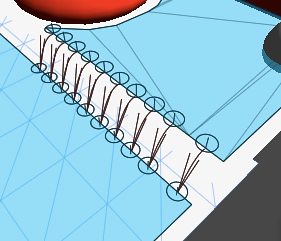
\includegraphics[width=0.3\textwidth]{images/OffMeshLinks-1.png}
	\caption{Off-Meshes links Beispiel aus Unity3D}
	\label{OffMeshesLinks}
	{\small{\it{Quelle: \cite{UnityDoc:np}}}}
\end{figure}

\subsection{Bewegung in Meshes}
Auf den Mesh-Polygonen k�nnen sich die Figuren in unterschiedlicher Weise orientieren. Es kommt darauf an, f�r die Situation geeignete Knoten auf den Polygonen zu setzen.
\begin{itemize}
\item \textbf{Polygon movement\\}
Die Knoten sitzen im Mittelpunkt der Dreiecke.\\
Da die Form die wenigsten Punkte benutzt, wird die CPU nicht zu arg belastet. Sie bietet dennoch ein nat�rliches Bewegungsmuster.
\item  \textbf{Edge movement\\}
Die Knoten sitzen auf den Kanten, die an andere Dreiecke schlie�en\\
Meist ist es unn�tig durch den Mittelpunkt aller Polygone zu gehen. Dieser Weg braucht mehr CPU-Leistung, sieht daf�r noch etwas realistischer aus.
\item \textbf{Vertex movement\\}
Die Knoten sitzen auf allen Eckpunkten\\
Der schnellste Weg geht meist direkt an einem Objekt vorbei. Mit dieser Mesh-Anordnung nimmt die Figur auch auf jeden Fall diese Route. Aber "'Wandschmuser"' hinterlassen nicht gerade das Bild eines realistischen Spielers.
\item \textbf{Hybrid movement\\}
Kombinationen der Oberen\\
Dies wird wohl die nat�rlichste Form der Spielerbewegung wiedergeben. Aber daf�r gibt es auch immer eine gr��ere Menge an Knoten zu berechnen, als wenn nur eine andere Form implementiert wird.\cite{Pat:mr}
\end{itemize}

\subsection{Pfadgl�ttung}
Egal welche Art von Mesh-Anordnung verwendet wird. Solange die Fortbewegungskosten konstant bleiben, kann man den Weg gerader machen.\\
So simuliert man zwar nicht NPC Verhalten in einer simulierten Welt, jedoch beispielsweise menschliches Gebaren f�r simulierte Gegner in Multiplayerspielen.
Ein Mensch w�rde, wenn er von A nach B kommen wollte, auf B zielen und nur den "'nach-vorne-Laufen"' Knopf bet�tigen. Es w�re ihm egal ob er an der Wand entlang schrammt oder sich dabei sonst wie nicht nat�rlich verh�lt.\\
Der benutzte Algorithmus ist dabei denkbar simpel.\\
Wenn man an Punkt $P_{i}$ steht und $P_{i+2}$ sichtbar ist, wird $P_{i+1}$ gel�scht. Wird dies oft genug wiederholt, besteht der Weg nur noch aus geraden Pfaden und den n�tigen Eckpunkten.\cite{Pat:mr}

\newpage
\section{Spielererfahrung}

Auf keinen Fall sollte es sich f�r den Spieler so anf�hlen, als w�rde der Computer cheaten, um zu gewinnen. Es l�sst sich durch die Mechanik der Programmierung jedoch fast nie vermeiden, dem KI-Gegner einen Vorsprung in Sachen taktischer Informationen zu gew�hren. Da der Computer das Spiel auf einer v�llig anderen Ebene interpretiert als der Mensch, sollte humanes Verhalten vom der KI simuliert werden.\\
Eine gute Methode ist Beispielsweise, in einem Spiel die generellen Gel�ndekosten f�r Felder zu erh�hen, die noch unerforscht sind. Obwohl dies f�r die KI offenkundig nie der Fall sein wird. So werden die gegnerischen Einheiten bevorzugt �ber aufgedecktes Gel�nde geschickt.
Nat�rlich sollte dieses Prinzip nicht f�r Einheiten gelten, welche erforschen sollen.\\
Am Ende soll es darauf hinaus laufen, dass der Gegner seine Einheiten wie ein menschlicher Spieler bewegt.\\
Ebenfalls darf der Spieler nicht der Meinung sein, dass seine Einheiten nicht seinen Befehle befolgt. \\
Eine sehr gute Methode zu verschleiern, was vor sich geht, ist die Einheit erst einmal in grober Richtung des Ziels aufbrechen und die Wegfindung bei niedrigster Priorit�t anlaufen zu lassen.
So wird dem Benutzer automatisch mitgeteilt, dass seine Befehle angekommen sind und die Steuerung funktioniert.\cite{Pat:ux}

\newpage
\section{Performance}
Die Hauptschleife von A* lie�t sich durch eine priorisierte Liste, analysiert und vertauscht dort Knoten. Ebenfalls werden die Knoten gespeichert, die schon besucht wurden.\\
Die Liste verk�rzen w�re nat�rlich die offensichtlichste L�sung um die Prozedur zu vereinfachen. Generell gilt: Wege �ber Meshes sind einfacher zu berechnen als �ber ein Grid, weil sie in der Regel weniger Knoten haben.\\
\subsection{Kartenhierarchie}
Wenn gr��ere Strecken zur�ckgelegt werden sollen, nehmen die ben�tigten Kosten zur Berechnung schnell �berhand. Eine gute Methode um dies zu vermeiden, ist eine vereinfachte, hierarchische Kartendarstellung zu erzeugen.\\
Generell kann man sich dieses Bewegungsmuster quasi so vorstellen, dass es auf gr��eren Welten etwas wie Bahnlinien gibt, an die sich die Figur halten kann. Kurz vor dem Ziel wird dieser Pfad verlassen und mit h�herer Aufl�sung nach dem besten Weg gesucht.
Zum Beispiel lassen sich in vielen Spielen H�user betreten und durch mehrere Zimmer beschreiten. Sitzt die Figur in einem Auto mit 120km/h auf der Autobahn, wird dies wohl nicht so schnell passieren.\\
Die Hierarchie muss ebenfalls nicht Homogen verlaufen. So kann man Grids und Meshes je nach Bedarf verwenden, vergr��ern oder vereinfachen.
Ist die Welt auf dem hierarchisch obersten Layer, kann an bestimmten, unver�nderlichen Punkten der einfachste Weg durch einen Bereich bereits errechnet sein. Alle Wege, die eine gewisse Komplexit�t unterschreiten, sind so in der h�chsten Aufl�sung bereits ermittelt.\cite{Pat:in}\\



%\chapter{Problemstellung}

Hier wird i.d.R. zun�chst das generell vorliegende Problem diskutiert: Was ist zu l�sen - was gibt
es bisher an L�sungsans�tzen (prinzipiell) und warum ist es wichtig, dass man dieses Problem l�st.
Letzteres ergibt sich oftmals aus der vorliegenden Anwendungssituation: Man braucht die L�sung, um
eine bestimmte Aufgabe zu erledigen, ein System aufzubauen etc. Der Bezug auf vorhandene oder auch
bisher fehlende L�sungen begr�ndet auch die Intension und Bedeutung dieser Arbeit. Dies k�nnen
allgemeine Gesichtspunkte sein - man liefert einen Beitrag f�r ein generell erkanntes oder zu
erkennendes Problem - oder man hat eben eine spezielle Systemumgebung oder Produkt (z.B. in einer
Firma u.s.w.), woraus sich dieses noch zu l�sende Problem ergibt.

Die genaue Problematik und Randbedingungen werden dann in Kapitel \hyperref[Aufgabenstellung]{Kapitel~\ref{Aufgabenstellung}}
dargestellt.
%\chapter{Aufgabenstellung und Zielsetzung}\label{Aufgabenstellung}

Hier wird nun die Aufgabenstellung konkret dargestellt: Was ist spezifisch zu l�sen? Welche
Randbedingungen sind prinzipiell gegeben und was ist die Zielsetzung? Letztere soll das
beschreiben, was man mit dieser Arbeit (mindestens) erreichen m�chte.
%\chapter{�brige Abschnitte (Kapitel und Abs�tze)}
Die Gliederung h�ngt nat�rlich vom Thema und von der L�sungsstrategie ab. Als n�tzliche
Anhaltspunkte k�nnen die Entwicklungsstufen oder - schritte z.B. der Softwareentwicklung betrachtet
werden. N�tzliche Gesichtspunkte erh�lt und erkennt man, wenn man sich
\begin{itemize}
  \item in die Rolle des Lesers oder
  \item in die Rolle des Entwicklers, der die Arbeit z.B. fortsetzen, erg�nzen oder pflegen soll,
\end{itemize}
versetzt. In der Regel wird vorausgesetzt, dass die Leser einen fachlichen Hintergrund haben - z.B.
Informatik studiert haben. D.h. nur in besonderen, abgesprochenen F�llen schreibt man in popul�rer
Sprache, so dass auch Nicht-Fachleute die Ausarbeitung prinzipiell lesen und verstehen k�nnen.

Die �u�ere Gestaltung der Ausarbeitung hinsichtlich Abschnittformate, Abbildungen, mathematische
Formeln usw. wird in \hyperref[Stile]{Kapitel~\ref*{Stile}} kurz dargestellt.
%\chapter{Latex-Bausteine}\label{Stile}

Der Text wird in bis zu drei Ebenen gegliedert:

\begin{enumerate}
  \item Kapitel ( \verb \chapter{Kapitel} ), \index{Kapitel}
  \item Unterkapitel  ( \verb \section{Abschnitt} ) und
  \item Unterunterkapitel  ( \verb \subsection{Unterabschnitte} ).
\end{enumerate}

\section{Abschnitt}\index{Abschnitt}
Text der Gliederungsebene 2.


\subsection{Unterabschnitt} \index{Unterabschnitt}
Text der Gliederungsebene 3.
Text Text Text Text Text Text Text Text Text Text Text Text Text Text Text
Beispiel f�r Quelltext\index{Quelltext} \\[2 ex]
\noindent
\begin{minipage}{1.0\textwidth} \small
\begin{lstlisting}
	Prozess 1:
	
	Acquire();
		a := 1;
	Release();
	...
	Acquire();
	if(b == 0)
	{					
		c := 3;
		d := a;
	}				
	Release();
\end{lstlisting}
\end{minipage}

\vspace{2cm}
\noindent
\begin{minipage}{1.0\textwidth} \small
\begin{lstlisting}
	Prozess 2:
	
	Acquire();
		b := 1;
	Release();
	...
	Acquire();
	if(a == 0)
	{					
		c := 5;
		d := b;
	}				
	Release();
\end{lstlisting}
\end{minipage}
\vskip 1em

Gr��ere Code-Fragmente sollten im Anhang eingef�gt werden.

\section{Abbildungen und Tabellen}

Abbildung\index{Abbildung} und Tabellen\index{Tabelle} werden zentriert eingef�gt. Grunds�tzlich sollen sie
erst dann erscheinen, nach dem sie im Text angesprochen wurden (siehe Abb. \ref{a1}). Abbildungen und Tabellen (siehe Tabelle \ref{t1}) k�nnen
im (flie�enden) Text (\verb here ), am Seitenanfang (\verb top ), am Seitenende
(\verb bottom ) oder auch gesammelt auf einer nachfolgenden Seite (\verb page )
oder auch ganz am Ende der Ausarbeitung erscheinen. Letzteres sollte man nur
dann w�hlen, wenn die Bilder g�nstig zusammen zu betrachten sind und die
Ausarbeitung nicht zu lang ist ($< 20$ Seiten).

\begin{figure} %[hbtp]
	\centering
		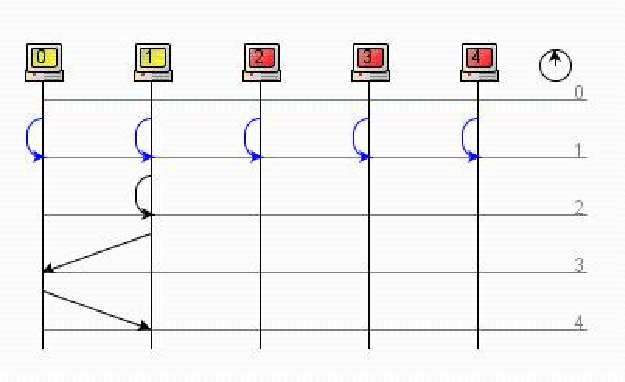
\includegraphics{images/p1ReadSeq.pdf}
	\caption{Bezeichnung der Abbildung}
	\label{a1}
\end{figure}

\begin{table} %[hbtp]
	\centering
		\begin{tabular}{l | l l l l}
		\textbf{Prozesse} & \textbf{Zeit} $\rightarrow$ \\
		\hline
			$P_{1}$ & $W(x)1$ \\
			$P_{2}$ & & $W(x)2$ \\
			$P_{3}$ & & $R(x)2$ & & $R(x)1$\\
			$P_{4}$ & & & $R(x)2$ & $R(x)1$\\
		\end{tabular}
	\caption{Bezeichnung der Tabelle}
	\label{t1}
\end{table}


\section{Mathematische Formel}\index{Formel}
Mathematische Formeln bzw. Formulierungen k�nnen sowohl im
laufenden Text (z.B. $y=x^2$) oder abgesetzt und zentriert im Text
erscheinen. Gleichungen sollten f�r Referenzierungen nummeriert
werden (siehe Formel \ref{gl-1}).
\begin{equation}
\label{gl-1}
e_{i}=\sum _{i=1}^{n}w_{i}x_{i}
\end{equation}

Entscheidungsformel:

\begin{equation}
\psi(t)=\left\{\begin{array}{ccc}
1 &  \qquad 0 <= t < \frac{1}{2} \\
-1 &  \qquad \frac{1}{2} <= t <1 \\
0 & \qquad sonst
\end{array} \right.
\end{equation}


Matrix:\index{Matrix}
\begin{equation}
A = \left(
\begin{array}{llll}
a_{11} & a_{12} & \ldots & a_{1n} \\
a_{21} & a_{22} & \ldots & a_{2n} \\
\vdots & \vdots & \ddots & \vdots \\
a_{n1} & a_{n2} & \ldots & a_{nn} \\
\end{array}
\right)
\end{equation}

Vektor:\index{Vektor} 

\begin{equation}
\overline{a} = \left(
\begin{array}{c}
a_{1}\\
a_{2}\\
\vdots\\
a_{n}\\
\end{array}
\right)
\end{equation}

\section{S�tze, Lemmas und Definitionen}\index{Satz}\index{Lemma}\index{Definition}

S�tze, Lemmas, Definitionen, Beweise,\index{Beweis} Beispiele\index{Beispiel} k�nnen in speziell daf�r vorgesehenen Umgebungen erstellt werden.

\begin{definition}(Optimierungsproblem)

Ein \emph{Optimierungsproblem} $\mathcal{P}$ ist festgelegt durch ein Tupel
$(I_\mathcal{P}, sol_\mathcal{P}, m_\mathcal{P}, goal)$ wobei gilt

\begin{enumerate}
\item $I_\mathcal{P}$ ist die Menge der Instanzen,
\item $sol_\mathcal{P} : I_\mathcal{P} \longmapsto \mathbb{P}(S_\mathcal{P})$ ist eine Funktion, die jeder Instanz $x \in I_\mathcal{P}$ eine Menge zul�ssiger L�sungen zuweist,
\item $m_\mathcal{P} : I_\mathcal{P} \times S_\mathcal{P} \longmapsto \mathbb{N}$ ist eine Funktion, die jedem Paar $(x,y(x))$ mit $x \in I_\mathcal{P}$ und $y(x) \in sol_\mathcal{P}(x)$ eine
Zahl $m_\mathcal{P}(x,y(x)) \in \mathbb{N}$ zuordnet (= Ma� f�r die L�sung $y(x)$ der Instanz $x$), und
\item $goal \in \{min,max\}$.
\end{enumerate}

\end{definition}

\begin{example} MINIMUM TRAVELING SALESMAN (MIN-TSP)
\begin{itemize}
\item $I_{MIN-TSP} =_{def}$ s.o., ebenso $S_{MIN-TSP}$
\item $sol_{MIN-TSP}(m,D) =_{def} S_{MIN-TSP} \cap \mathbb{N}^m$ 
\item $m_{MIN-TSP}((m,D),(c_1, \ldots , c_m)) =_{def} \sum_{i=1}^{m-1} D(c_i, c_{i+1}) + D(c_m,c_1)$ 
\item $goal_{MIN-TSP} =_{def} min$
\end{itemize}
\begin{flushright}
$\qed$
\end{flushright}
\end{example}

\begin{theorem} Sei $\mathcal{P}$ ein \textbf{NP}-hartes Optimierungsproblem.
Wenn $\mathcal{P} \in$ \textbf{PO}, dann ist \textbf{P} = \textbf{NP}.
\end{theorem}

\begin{proof} Um zu zeigen, dass \textbf{P} = \textbf{NP} gilt, gen�gt es
wegen Satz A.30 zu zeigen, dass ein einziges \textbf{NP}-vollst�ndiges
Problem in \textbf{P} liegt. Sei also $\mathcal{P}'$ ein beliebiges \textbf{NP}-vollst�ndiges Problem.

Weil $\mathcal{P}$ nach Voraussetzung \textbf{NP}-hart ist, gilt insbesondere
$\mathcal{P}' \leq_T \mathcal{P}_C$. Sei $R$ der zugeh�rige
Polynomialzeit-Algorithmus dieser Turing-Reduktion.
Weiter ist $\mathcal{P} \in$ \textbf{PO} vorausgesetzt, etwa verm�ge eines
Polynomialzeit-Algorithmus $A$. Aus den beiden
Polynomialzeit-Algorithmen $R$ und $A$ erh�lt man nun
leicht einen effizienten Algorithmus f�r $\mathcal{P}'$: Ersetzt man
in $R$ das Orakel durch $A$, ergibt dies insgesamt eine polynomielle
Laufzeit. 
%\begin{flushright}
$\qed$
% \end{flushright}
\end{proof}

\begin{lemma} Aus \textbf{PO} $=$ \textbf{NPO} folgt \textbf{P} $=$ \textbf{NP}.
\end{lemma}

\begin{proof} Es gen�gt zu zeigen, dass unter der angegeben
Voraussetzung KNAPSACK $\in$ \textbf{P} ist.

Nach Voraussetung ist MAXIMUM KNAPSACK $\in$ \textbf{PO},
d.h. die Berechnung von $m^*(x)$ f�r jede Instanz $x$ ist
in Polynomialzeit m�glich. Um KNAPSACK bei Eingabe
$(x,k)$ zu entscheiden, m�ssen wir nur noch $m^*(x) \geq k$
pr�fen. Ist das der Fall, geben wir $1$, sonst $0$ aus. Dies
bleibt insgesamt ein Polynomialzeit-Algorithmus. 
\begin{flushright}
$\qed$
\end{flushright}
\end{proof}

\section{Fu�noten}

In einer Fu�note k�nnen erg�nzende Informationen\footnote{Informationen die f�r die Arbeit zweitrangig sind, jedoch f�r den Leser interessant sein k�nnten.} angegeben werden. Au�erdem kann eine Fu�note auch Links enthalten. Wird in der Arbeit eine Software (zum Beispiel Java-API\footnote{\url{http://java.sun.com/}}) eingesetzt, so kann die Quelle, die diese Software zur Verf�gung stellt in der Fu�note angegeben werden.

\section{Literaturverweise}\index{Literatur}
Alle benutzte Literatur wird im Literaturverzeichnis angegeben\footnote{Dazu wird ein sogennanter bib-File, literatur.bib verwendet.}. Alle angegebene Literatur sollte mindestens einmal im Text referenziert werden\cite{Coulouris:02}.
%% To structure your document use chapter->section->subsection ...

\chapter{Beispiel-Kapitel}

In diesem Kapitel wird beschrieben, warum es unterschiedliche Konsistenzmodelle\index{Konsistenzmodelle} gibt. Au�erdem werden die Unterschiede zwischen strengen Konsistenzmodellen\index{Linearisierbarkeit} (Linearisierbarkeit, sequentielle Konsistenz)\index{sequentiell!Konsistenz} und schwachen Konsistenzmodellen\index{Konsistenz!schwach} (schwache Konsistenz, Freigabekonsistenz)\index{Freigabekonsistenz} erl�utert. Es wird gekl�rt, was Strenge und Kosten (billig, teuer) in Zusammenhang mit Konsistenzmodellen bedeuten.

\section{Warum existieren unterschiedliche Konsistenzmodelle?}

Laut \cite{Malte:97} sind mit der\index{Replikation} Replikation von Daten immer zwei gegens�tzliche Ziele verbunden: die Erh�hung der\index{Verf�gbarkeit} Verf�gbarkeit und die Sicherung der\index{Konsistenz} Konsistenz der Daten. Die Form der Konsistenzsicherung bestimmt dabei, inwiefern das eine Kriterium erf�llt und das andere dementsprechend nicht erf�llt ist (Trade-off zwischen Verf�gbarkeit und der Konsistenz der Daten). Stark konsistente Daten sind stabil, das hei�t, falls mehrere Kopien der Daten existieren, d�rfen keine Abweichungen auftreten. Die Verf�gbarkeit der Daten ist hier jedoch stark eingeschr�nkt. Je schw�cher die Konsistenz wird, desto mehr Abweichungen k�nnen zwischen verschiedenen Kopien einer Datei auftreten, wobei die Konsistenz nur an bestimmten Synchronisationspunkten gew�hrleistet wird. Daf�r steigt aber die Verf�gbarkeit der Daten, weil sie sich leichter replizieren lassen.

Nach \cite{Mosberger:93} kann die Performanzsteigerung der schw�cheren Konsistenzmodelle wegen der Optimierung\index{Optimierung} (Pufferung, Code-Scheduling, Pipelines) 10-40 Prozent betragen. Wenn man bedenkt, dass mit der Nutzung der vorhandenen Synchronisierungsmechanismen schw�chere Konsistenzmodelle den Anforderungen der strengen Konsistenz gen�gen, stellt sich der h�here programmiertechnischer Aufwand bei der Implementierung der schw�cheren Konsistenzmodelle als ihr einziges Manko dar.

In \cite{Cheriton:85} ist beschrieben, wie man sich Formen von DSM vorstellen k�nnte, f�r die ein beachtliches Ma� an\index{Inkonsistenz} Inkonsistenz akzeptabel w�re. Beispielsweise k�nnte DSM verwendet werden, um die Auslastung von Computern in einem Netzwerk zu speichern, so dass Clients f�r die Ausf�hrung ihrer Applikationen die am wenigsten ausgelasteten Computer ausw�hlen k�nnen. Weil die Informationen dieser Art innerhalb k�rzester Zeit ungenau werden k�nnen (und durch die Verwendung der veralteten Daten keine gro�en Nachteile entstehen k�nnen), w�re es vergebliche M�he, sie st�ndig f�r alle Computer im System konsistent zu halten \cite{Coulouris:02}. Die meisten Applikationen stellen jedoch strengere Konsistenzanforderungen.

\section{Klassifizierung eines Konsistenzmodells}

Die zentrale Frage, die f�r die Klassifizierung\index{streng}\index{schwach} (streng oder schwach) eines Konsistenzmodells von Bedeutung ist \cite{Coulouris:02}: wenn ein Lesezugriff auf eine Speicherposition erfolgt, welche Werte von Schreibzugriffen auf diese Position sollen dann dem Lesevorgang bereitgestellt werden? Die Antwort f�r das schw�chste Konsistenzmodell lautet: von jedem Schreibvorgang, der vor dem Lesen erfolgt ist, oder in der "`nahen"' Zukunft, innerhalb des definierten Betrachtungsraums, erfolgten wird. Also irgendein Wert, der vor oder nach dem Lesen geschrieben wurde.

F�r das strengste Konsistenzmodell, Linearisierbarkeit (atomic consistency), stehen alle geschriebenen Werte allen Prozessoren sofort zur Verf�gung: eine Lese-Operation gibt den aktuellsten Wert zur�ck, der geschrieben wurde, bevor das Lesen stattfand. Diese Definition ist aber in zweierlei Hinsicht problematisch. Erstens treten weder Schreib- noch Lese-Operationen zu genau einem Zeitpunkt auf, deshalb ist die Bedeutung von "`aktuellsten"' nicht immer klar. Zweitens ist es nicht immer m�glich, genau festzustellen, ob ein Ereignis vor einem anderen stattgefunden hat, da es Begrenzungen daf�r gibt, wie genau Uhren in einem verteilten System synchronisiert werden k�nnen.

Nachfolgend werden einige Konsistenzmodelle absteigend nach ihrer Strenge vorgestellt. Zuvor m�ssen wir allerdings kl�ren, wie die Lese- und Schreibe-Operationen in dieser Ausarbeitung dargestellt werden.

Sei $x$ eine Speicherposition, dann k�nnen Instanzen dieser Operationen wie folgt ausgedr�ckt werden:
\begin{itemize}
	\item $R(x)a$ - eine Lese-Operation\index{Operation!Lese}, die den Wert $a$ von der Position $x$ liest.
	\item $W(x)b$ - eine Schreib-Operation\index{Operation!Schreib}, die den Wert $b$ an der Position $x$ speichert.
\end{itemize}

\section{Linearisierbarkeit\index{Linearisierbarkeit} (atomic consistency)}

Die Linearisierbarkeit im Zusammenhang mit DSM kann wie folgt definiert werden:
\begin{itemize}
	\item Die verzahnte Operationsabfolge findet so statt: wenn $R(x)a$ in der Folge vorkommt, dann ist die letzte Schreib-Operation, die vor ihr in der verzahnten Abfolge auftritt, $W(x)a$, oder es tritt keine Schreib-Operation vor ihr auf und $a$ ist der Anfangswert von $x$. Das bedeutet, dass eine Variable nur durch eine Schreib-Operation ge�ndert werden kann.
	\item Die Reihenfolge der Operationen in der Verzahnung ist konsistent zu den \underline{Echtzeiten}\index{Echtzeiten}, zu denen die Operationen bei der tats�chlichen Ausf�hrung aufgetreten sind.
\end{itemize}

Die Bedeutung dieser Definition kann an folgendem Beispiel (Tabelle \ref{tab:1}) nachvollzogen werden. Es sei angenommen, dass alle Werte mit $0$ vorinitialisiert sind.

\begin{table}
	\centering
		\begin{tabular}{l | l l l l}
			\textbf{Prozesse} & \textbf{Zeit} $\rightarrow$ & \\
			\hline
			$P_{1}$ & $W(x)1$ & & $W(y)2$ \\
			$P_{2}$ & & $R(x)1$ & & $R(y)2$ \\
		\end{tabular}
	\caption{Linearisierbarkeit ist erf�llt}
	\label{tab:1}
\end{table}

Hier sind beide Bedingungen erf�llt, da die Lese-Operationen den zuletzt geschriebenen Wert zur�ckliefern. Interessanter ist es, zu sehen, wann die Linearisierbarkeit verletzt ist.

\begin{table}
	\centering
		\begin{tabular}{l | l l l l}
		\textbf{Prozesse} & \textbf{Zeit} $\rightarrow$ \\
		\hline
		$P_{1}$ & $W(x)1$ & $W(x)2$ \\
		$P_{2}$ & & & \color{red} $R(x)0$ & \color{black} $R(x)2$ \\
		\end{tabular}
	\caption{Linearisierbarkeit ist verletzt, sequentielle Konsistenz ist erf�llt.}
	\label{tab:2}
\end{table}

In diesem Beispiel (Tabelle \ref{tab:2}) ist die Echtzeit-Anforderung verletzt, da der Prozess $P_{2}$ immer noch den alten Wert liest, obwohl er von Prozess $P_{1}$ bereits ge�ndert wurde. Diese Ausf�hrung w�re aber sequentiell konsistent (siehe kommender Abschnitt), da es eine Verzahnung der Operationen gibt, die diese Werte liefern k�nnte ($R(x)0$, $W(x)1$, $W(x)2$, $R(y)2$). W�rde man beide Lese-Operationen des 2. Prozesses vertauschen, wie in der Tabelle \ref{tab:3} dargestellt, so w�re keine sinnvolle Verzahnung mehr m�glich.

\begin{table}
	\centering
		\begin{tabular}{l | l l l l}
		\textbf{Prozesse} & \textbf{Zeit} $\rightarrow$ \\
		\hline
		$P_{1}$ & $W(x)1$ & $W(x)2$ \\
		$P_{2}$ & & & \color{red} $R(x)2$ &  \color{red} $R(x)0$ \\
			
		\end{tabular}
	\caption{Linearisierbarkeit und sequentielle Konsistenz sind verletzt.}
	\label{tab:3}
\end{table}

In diesem Beispiel sind beide Bedingungen verletzt. Selbst wenn die Echtzeit, zu der die Operationen stattgefunden haben, ignoriert wird, gibt es keine Verzahnung einzelner Operationen, die der Definition entsprechen w�rde.
% ...

%--------------------------------------------------------------------------
\backmatter                        %Anhang
%-------------------------------------------------------------------------
%Literaturverzeichnis - notwendig
%Literaturverzeichnis - notwendig
% - use bibstyle 'geralpha', 'gerplain', ...
%\bibliographystyle{gerplain}
\bibliographystyle{geralpha}
\bibliography{literatur}     %BibTeX-File literatur.bib
%--------------------------------------------------------------------------
\printindex % Index ausdr�cken - optional
%--------------------------------------------------------------------------
% Anh�nge sind optional
\begin{appendix}
   \chapter{Glossar}

%geordnete tabelle, 2spaltig?
%\listofabbreviations
\abbreviation{DisASTer}		{DisASTer (Distributed Algorithms Simulation Terrain) A platform for the Implementation of Distributed Algorithms}
\abbreviation{DSM}		{		Distributed Shared Memory}
\abbreviation{AC}		{		Linearisierbarkeit (atomic consistency)}
\abbreviation{SC}		{		Sequentielle Konsistenz (sequential consistency)}
\abbreviation{WC}		{		Schwache Konsistenz (weak consistency)}
\abbreviation{RC}		{		Freigabekonsistenz (release consistency)}
   
   \chapter{Erkl�rung der Kandidatin / des Kandidaten}

\begin{description}[$\Box$~]
\item[$\Box$] Die Arbeit habe ich selbst�ndig verfasst und keine anderen als die angegebenen Quellen- und Hilfsmittel verwendet.\\

\item[$\Box$] Die Arbeit wurde als Gruppenarbeit angefertigt. Meine eigene Leistung ist ... \\
...\\

Diesen Teil habe ich selbst�ndig verfasst und keine anderen als die angegebenen Quellen und Hilfsmittel verwendet. \\

Namen der Mitverfasser: ...

\end{description}

\vspace{2cm}

\begin{minipage}[t]{3cm}
\rule{3cm}{0.5pt}
Datum
\end{minipage}
\hfill
\begin{minipage}[t]{9cm}
\rule{9cm}{0.5pt}
Unterschrift der Kandidatin / des Kandidaten
\end{minipage} 
\end{appendix}
\end{document}
